\documentclass[12pt, letterpaper]{article} 
\usepackage[utf8]{inputenc}
\usepackage{setspace}
\usepackage[spanish]{babel} %pone en español textos automaticos
\usepackage{fancyhdr} % Se agrega el paquete fancyhdr
\usepackage{graphicx} % Se agrega el paquete graphicx
\usepackage{float} %para agregar imagenes con H
\usepackage{pdfpages} %agregar pdfs para datasheets y eso
\usepackage[a4paper, margin=3cm]{geometry} %marjenes y hoja A4


%pies de pagina
\pagestyle{fancy} % Se especifica el estilo de página como fancy
\fancyhf{} % Se limpian los encabezados y pies de página predefinidos
\rfoot{Página \thepage\ de \pageref{LastPage}} %texto derecha
\lfoot{Medidas Electrónicas I} %texto izquierda
%encabezado de pagina
\chead{UNIVERSIDAD TECNOLÓGICA NACIONAL - FRC} % centro
\fancyhead[R]{
\includegraphics[height=1cm]{imagenes/UTN_logo.jpg}}


\begin{document}

%Caratula
\begin{titlepage}
	\centering %texto centrado
	{
\includegraphics[width=0.2\textwidth]{imagenes/UTN_logo.jpg}\par}
	{\bfseries\LARGE Universidad Tecnológica Nacional \par}
	{\scshape\Large Facultad Regional Córdoba\par}
	\vspace{0.5cm}
	{\scshape\Huge Trabajo Práctico de laboratorio Nro. 2  \par}%titulo
	\raggedright %texto a la izquierda
	\vspace{0.5cm}
	{\Large Materia: Medidas Electrónicas 1 \par}%Materia
	\vspace{0.5cm}
	{\Large Curso: 4R1 \par}
	\vspace{0.5cm}
	{\Large Edificio: \par}%edificios
	\begin{itemize}
		\item{\Large Ingeniero Soro [Aula 606] \par}
		\item{\Large Laboratorio de electrónica \par}
	\end{itemize}
	\vspace{0.5cm}
	{\Large Profesores: \par} %profes
	\begin{itemize}
		\item{\Large [Teórico] Ing, Carlos Augusto Centeno \par}
		\item{\Large [Teórico] Ing, Luis Alberto Guanuco \par}
		\item{\Large [Práctico] Ing, Martin Alejandro Salamero \par}
	\end{itemize}
	\vspace{0.5cm}
	{\Large Autores: \par} %autores
	\begin{itemize}
		\item{\Large Pappano Meinardi, Joaquín - Leg.86730\par}
		\item{\Large Monteros Vigueras, Juan Manuel - Leg.86334\par}
		\item{\Large Romero Diaz, Agustín - Leg.86821\par}
	\end{itemize}
	\vspace{0.5cm}
	{\Large Fecha: {\today} \par}%pone fecha de hoy
\end{titlepage}

%Indice
\newpage
\tableofcontents
\newpage
%cuerpo documento
\section{Introducción}

La medida de la resistencia de un cable conductor se realiza mediante 
el método de 4 terminales.Cuando se realiza la medición de resistencia
de pequeño valor con el ohmetro de un multímetro comun, se tiene en cuenta
que el resultado obtenido puede estar afectado de un error importante
por la presencia de resistencias de contactos entre las terminales del
elemento a medir y las puntas de la prueba del instrumento. Estas resistencias
de contacto son de valor impredecible y por ende resulta muy difícil descontar 
el error. 
\singlespacing
Para la medición de la resistencia de un sistema puesta a tierra,se realiza 
también un método que emplea una fuente de corriente constante, es el de la "resistencia
de sistema puesta a tierra". El tipo de instrumento que se utiliza se conoce como
"Telurimetro", y permite hacer la medición de forma directa. Se entiende como “sistema de puesta a tierra” 
a la conección que se efectúa mediante un electrodo metálico,jabalina, que se inserta en el suelo y 
que se emplea como punto de retorno en diversos tipos de sistemas, (instalaciones de energía 
eléctrica; sistema de descarga atmosféricas; plano de tierra de antenas etc..).

\subsection{Objetivo}
Determinar el valor de la resistencia en situaciones específicas. Dar el resultado de la
medición acompañado del grado de incertidumbre.

\subsection{Materiales e Instrumental}
\begin{itemize}
	\item Multímetro digital UNI-T UT39C+.
	\item Circuito generador de corriente constante.
	\item Probeta a ensayar (Tramo de cable o alambre de longitud conocida).
	\item Telurimetro UNI-T Modelo UT522 (Con su juego de cables, electrodos y accesorios)
\end{itemize}

\section{Primer parte - Medición de la resistencia de un cable conductor}

\begin{figure}[H]
	\centering
	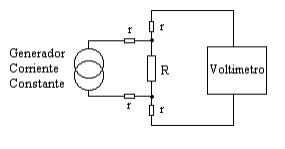
\includegraphics{imagenes/met_4_terminales.jpg}
	\caption{Método cuatro terminales}
    \label{fig:met_4_terminales}
\end{figure}

Se puede efectuar una medición más exacta de resistencias de pequeño valor, utilizando el método de 4 terminales. 
Este método se vale de una fuente que proporciona una corriente constante de prueba, la cual se aplica al elemento cuya resistencia
se desea medir por medio de dos terminales, luego se determina la caída de tensión provocada
mediante un voltímetro que se conecta con otros dos terminales separados de los primeros.
Las resistencias de contacto no se eliminan, pero al separarse los "contactos de corriente" y
los "contactos de potencial", el error puede ser anulado.
\singlespacing
En esta parte del trabajo práctico se determinará la resistencia total de un
trozo de cable/alambre conductor, mediante el empleo del método descrito. 
\singlespacing

\subsection{Procedimiento}

\begin{enumerate}
	\item Se coloca el generador de corriente constante fijo a un valor de 100mA.Para esto se emplea un circuito con un regulador monolítico
	LM317 (\ref{fig.gen_corriente}), este se coloca a una tensión de entrada de 12v para asegurar su funcionamiento.
	
	\begin{figure}[H]
		\centering
		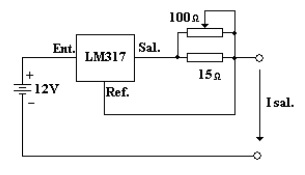
\includegraphics{imagenes/circuito_lm317.jpg}
		\caption{Circuito generador de corriente constante}
        \label{fig.gen_corriente}
	\end{figure}

	\item Se colocan los extremos de la Probeta (tramo de conductor) conectados a la fuente de corriente. la misma esta en un arrollamiento no inductivo, el cual se consigue plegando el cable por la mitad y luego arrollando el conjunto.
 \item Con ayuda de un multimetro con amperímetro, para el caso se utilizo un UNI-T UT39C+, se regula el generador de corriente a 100mA.
 \item Se conecta la probeta a medir al generador cerrando así el circuito.
 \item Se mide a bornes de la probeta la caída de tensión con un multimetro como voltímetro, para el caso se utilizo un UNI-T UT39C+.
 \item Utilizando la ley de ohm se calcula la resistencia en el cable.
$V=R*I$
\end{enumerate}

\subsection{Valores obtenidos}
\begin{table}[H]
    \centering
    \caption{Valores obtenidos y calculados}
    \begin{tabular}{|c|c}\hline
     --   & Valores \\\hline
     V   & 103.6mV   \\ \hline   
     I    &  100mA   \\ \hline
    R   & 1.035$\Omega$  \\ \hline 
    \end{tabular}
    \label{tab:tab_medidas}
\end{table}

\subsection{Cálculo de la incertidumbre en la medición}

La incertidumbre en la determinación de la resistencia por el método propuesto, se vincula con los 
errores que pueden estar presentes en cada una de las mediciones implicadas en el procedimiento. En 
este caso hay dos mediciones que se han efectuado, una de corriente y una de tensión, y las dos se 
hacen con el multímetro. El valor de la resistencia resulta ser el cociente entre la tensión y la 
corriente, por ende el error relativo máximo total es la suma de los errores relativos máximos parciales.
\singlespacing
\begin{figure}[H]
		\centering
		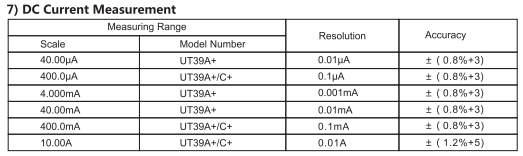
\includegraphics{imagenes/DC_ut39c.png}
		\caption{Especificaciones para corriente continua UT39C+}
        \label{fig:DC_UT39C}
	\end{figure}
 \begin{figure}[H]
		\centering
		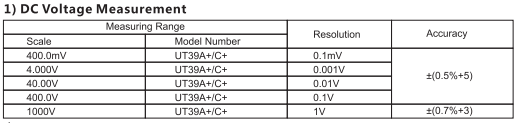
\includegraphics{imagenes/DV_ut39c.png}
		\caption{Especificaciones para voltaje en continua UT39C+}
        \label{fig:DV_UT39C}
	\end{figure}
$\frac{\Delta R}{R} = \frac{\Delta V}{V}+\frac{\Delta I}{I}$

\singlespacing
Los errores máximos parciales (o incertidumbre) para cada una de las mediciones se deben 
obtener de las especificaciones de exactitud del multímetro empleado. 
\singlespacing
$\Delta X=( \frac{\textbf{Valor promedio \%}}{100} + N° digitos)$
\singlespacing
%POner el + arriba del -%
En este caso se uso una escala de tantos V con una exactitud $\pm$ (0,5\% + 5 digitos) y para una escala de 400mA una exactitud de $\pm$(0,8\% + 3 dígitos)
por lo que podemos calcular los valores de incertidumbre y errores relativos.
\singlespacing  

\item  Incertidumbres\singlespacing
$\Delta I= \frac{0,8 * 100mA}{100}+0.3mA=1,1mA$\singlespacing
$\Delta V= \frac{0,5 * 103,6mV}{100}+0.5mV=1,018mV$\singlespacing
\item Errores Relativos\singlespacing
$\frac{\Delta V}{V}=9,826*10^{-3}$\singlespacing
$\frac{\Delta I}{I}=11*10^{-3}$ \singlespacing
\item Calculo de la incertidumbre en la resistencia\singlespacing

$\frac{\Delta R}{R} =\frac{\Delta V}{V} + \frac{\Delta I}{I}$ \singlespacing
$\frac{\Delta R}{R}=9,826*10^{-3}+11*10^{-3}=20.826*10^{-3}$
$\Delta R * R=21.52*10^{-3}$\singlespacing

\item Errores relativos Porcentuales\singlespacing

$\frac{\Delta V}{V} * 100=0.982\%$\singlespacing
$\frac{\Delta I}{I} * 100=1.1\%$\singlespacing
$\frac{\Delta R}{R} * 100=2.082\%$\singlespacing
 
\begin{table}[H]
\centering
\caption{Incertidumbres en la medición}
	\begin{tabular}{|c|c|c|c|c|}
    	\hline
    	----------- & ----------- & $\Delta x$  & $\frac{\Delta x}{X}$  & $\frac{\Delta x}{X} *100$ \\ \hline
    	V           & 103,6 mV    & 1,018mV & 9,826      & 0,982\%        \\ \hline
    	I           & 100 mA      & 1,1mA   & 11         & 1,1\%          \\ \hline
    	R           & 1,036    $\Omega$    & 21,016 $\Omega$  & 20,286     & 2,028\%        \\ \hline
	\end{tabular}
 \label{tab\insertidumbres}
\end{table}

\singlespacing
\section{Segunda parte - Medición de la resistencia de un sistema de puesta a tierra (Jabalina)}
una medición habitual que implementa un método indirecto de cuatro terminales es el de la resistencia de “sistemas de puesta a tierra”. El tipo de
instrumento que se utiliza se conoce como Telurimetro (figura \ref{fig:telurimetro}). Se entiende como “sistema de puesta a tierra” a la coneccion que se efectúa
mediante un electrodo metálico (“jabalina” o “malla conductora”) que se inserta en el suelo y
que se emplea como punto de retorno en diversos tipos de sistemas, (instalaciones de energia
electrica; sistema de descarga atmosfericas; plano de tierra de antenas etc..).
La resistencia de un sistema de puesta a tierra, consiste en la suma de la resistencia propia del
electrodo (valor muy bajo) más la resistencia de contacto entre
el mismo y la tierra propiamente dicha. Aunque la resistividad del suelo puede ser variable.
Si se hace circular una corriente I entre dos electrodos de puesta a tierra a y b separados entre si, la caída de tensión a lo largo de la linea que une a los mismos, medida con un
voltímetro y un tercer electrodo que se desplaza sobre la linea, presenta la
siguiente distribución. (figura \ref{fig:med_puesta_tie}).

\begin{figure}[H]
	\centering
	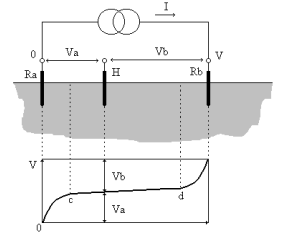
\includegraphics[width=0.6\textwidth]{imagenes/medida_puesta_t.png}
	\caption{Circuito medición puesta tierra}
	\label{fig:med_puesta_tie}
\end{figure}
\singlespacing
Un Telurimetro consiste básicamente en un aparato de medición que contiene un Voltímetro cuya lectura esta calibrada directamente en ohm, y una fuente de corriente alterna constante de baja frecuencia (no puede ser de corriente continua por los efectos de polarización
que se producirían debido a las reacciones electrolíticas). Además, la frecuencia debe ser diferente de la frecuencia de la red eléctrica para evitar la interferencias.
\singlespacing
\begin{figure}[H]
	\centering
	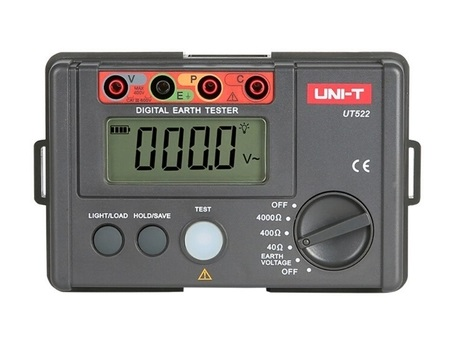
\includegraphics[width=0.75\textwidth]{imagenes/Telerimetro_UNIT.jpg}
	\caption{Telurimetro UNI-T UT522}
	\label{fig:telurimetro}
\end{figure}
\subsection{Procedimiento}

Para la medición de la resistencia de un sistema de puesta a tierra, se deberían
insertar en el terreno los electrodos auxiliares y conectarlos al Telurimetro empleando los
cables correspondientes conforme se indica en la figura \ref{fig:conexion_telurimetro} brindada por el fabricante del instrumento.
\begin{figure}[H]
	\centering
	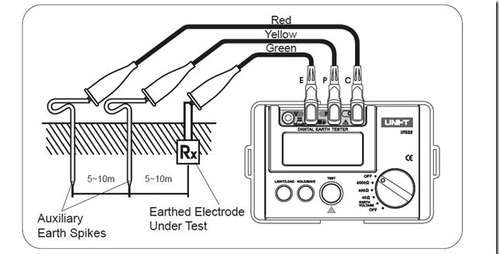
\includegraphics[width=0.75\textwidth]{imagenes/conexion_telurimetro.jpg}
	\caption{Conexión telurimetro UNI-T UT522}
	\label{fig:conexion_telurimetro}
\end{figure}
\subsection{Pasos realizados}
\begin{enumerate}
    \item se conecta el cable Verde del telerimetro a la puesta tierra o jabalina a medir. Por norma esta debe ser accesible a través de una caja de mantenimiento si ya se encuentra colocada.
    \item se extienden a toda su longitud  los cables Amarillo y Rojo donde este ultimo sera el mas largo, esto también puede verse aclarado en la figura \ref{fig:conexion_telurimetro}. 
    \item Cada uno de los cables desplegados debe ser unido a tierra mediante un electrodo que se incluye en el instrumento. Es importante que tanto los electrodos colocados como la jabalina se encuentren sobre una misma linea recta. Cabe aclarar que en la medición dentro del laboratorio se emplearon electrodos auxiliares por la imposibilidad de clavar en la tierra, estos conciten en una pesa unida al piso por un paño húmedo.  ver en  figura  \ref{fig:electrodo}.
\begin{figure}[H]
	\centering
	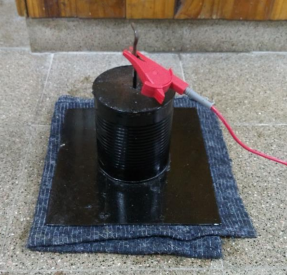
\includegraphics[width=0.5\textwidth]{imagenes/electrodo_aux.png}
	\caption{Electrodo auxiliar utilizado en interiores}
	\label{fig:electrodo}
\end{figure}
\item Con el selector rotativo, seleccionar inicialmente el rango de 4000 $\Omega$.
\item Se pulsa el botón identificado como “TEST” lo que visualiza el valor obtenido. Para los casos puestos en practica se cambio en este punto la escala de rango a los 40 $\Omega$ para así tener mejor lectura de los valores.
\item En caso de que algún cable no realice correcta conexión el telurimetro nos indicara en pantalla que el circuito se halla abierto.
\end{enumerate}
\singlespacing

\subsection{Valores obtenidos}
\begin{itemize}
    \item $laboratorio \rightarrow R(jabalina)=2,93 \Omega$
    \item $Patio \rightarrow R(jabalina)=0,27 \Omega$
\end{itemize}

\subsection{Incertidumbre Telurimetro}
Calculo de incertidumbre en las mediciones teniendo en cuenta los datos brindados en el manual de usuario del telurimetro utilizado. ver en figura \ref{fig:epecificacion_telur}.
\begin{figure}[H]
	\centering
	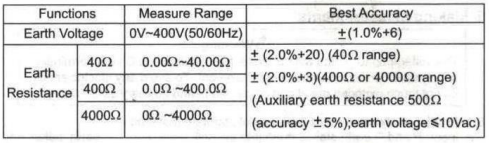
\includegraphics[width=0.75\textwidth]{imagenes/especificaciones_telurimetro.png}
	\caption{Especificaciones UNI-T UT522}
	\label{fig:epecificacion_telur}
\end{figure}
$\Delta Rj(laboratorio)=\frac{2*2,93\Omega}{100}+0,2\Omega=0,2586$
\singlespacing
$\Delta Rj(patio)=\frac{2*0,27\Omega}{100}+0,2\Omega=0,2079$
\singlespacing
$Rj(laboratorio) = (2,93\pm0,2586)\Omega$
\singlespacing
$Rj(patio) = (0,27\pm0,2079)\Omega$


\section{Conclusiones}

Leer bien que pide el tp acá

\newpage
\section{Anexo}

\begin{figure}[H]
    \centering
    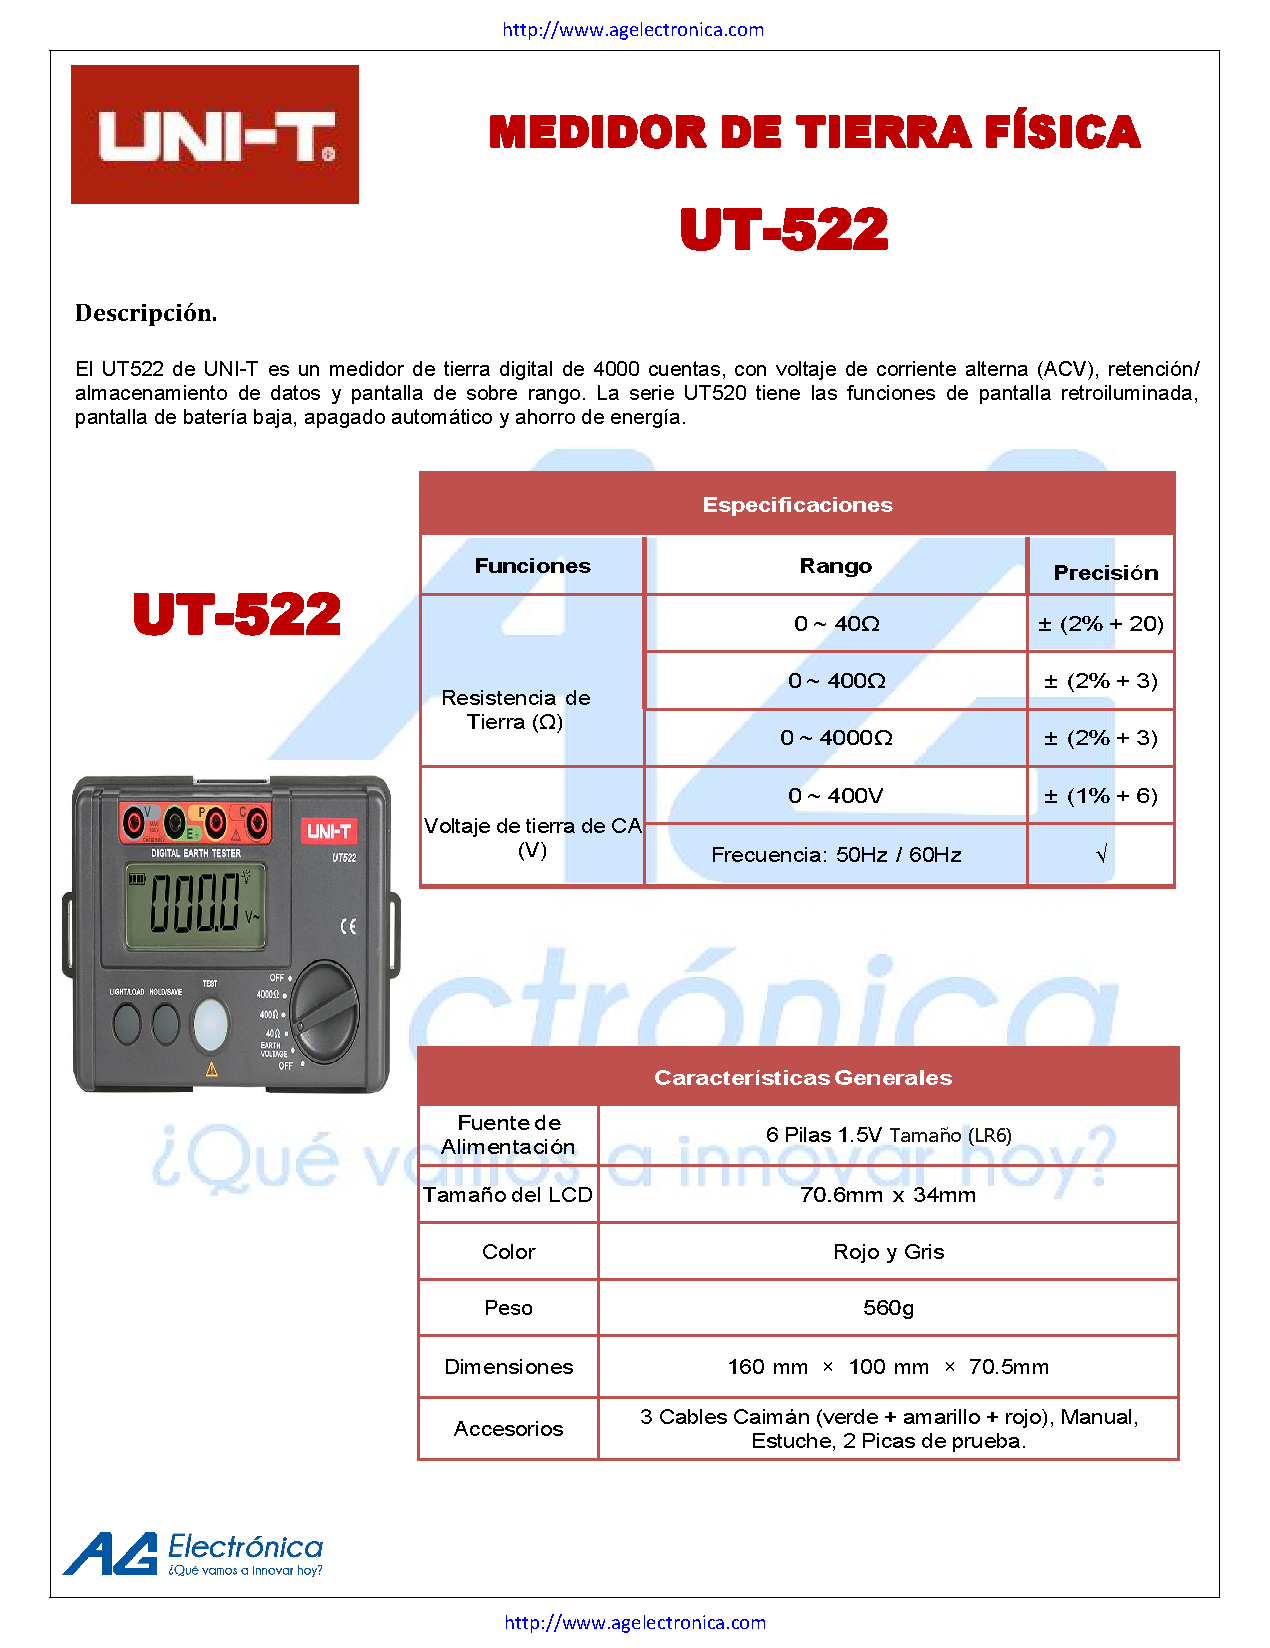
\includepdf[pages={1}, scale=0.60 ,pagecommand={\pagestyle{fancy}\fancyhf{}}]{imagenes/UT-522.pdf}
    \caption{Manual telurimetro UNI-T UT522}
    \label{fig:manual_UT522}
\end{figure}
\newpage
\begin{figure}[H]
    \centering
    \includepdf[pages={2}, scale=0.80 ,pagecommand={\pagestyle{fancy}\fancyhf{}}]{imagenes/UT-522.pdf}
    \caption{Manual telurimetro UNI-T UT522}
\end{figure}
\newpage
\begin{figure}[H]
    \centering
    \includepdf[pages={2}, scale=0.80 ,pagecommand={\pagestyle{fancy}\fancyhf{}}]{imagenes/UT39C.pdf}
    \caption{Manual multimetro UNI-T UT39C+}
    \label{fig:manual_UT39c}
\end{figure}

\label{LastPage}
\end{document}